\documentclass[11pt]{article}
\usepackage{fullpage}
\usepackage{amsmath}
\usepackage{esint}
\usepackage{tabularx} 
\usepackage{cancel}
\usepackage{graphicx}
\linespread{1.1}


\begin{document}

\title{BME205 \\ Fundamentals of Biomedical Engineering}
\author{Michael Boyadjian}
\maketitle
\pagebreak

\tableofcontents

\pagebreak

\bigskip
\bigskip
\bigskip

\section{Foundation of Physiology}

\subsection{Homoeostasis}
Homoeostasis is the ability of a cell or organism to regulate its internal conditions typically using feedback systems to minimize variation and maintain health regardless of changes in external environment.

\subsubsection{Body Cells}
The fluid collectively contained within all body cells is known as \textbf{intercellular fluid (ICF)}. The fluid outside the cells is called \textbf{extracellular fluid (ECF)}. Extracellular fluid is made up of two components: \textbf{plasma}, the fluid component of blood; and \textbf{interstitial fluid}, which surrounds and bathes the cells

\subsubsection{Body Systems}
Homoeostasis is essential for the survival of each cell, and each cell, through its specialized activities, contributes as part of a body system to the maintenance of the internal environment shared by all cells. It is not a rigid, fixed state, or absolute setting, but rather a dynamic, steady state in which changes occur but are minimized by multiple dynamic equilibrium adjustment mechanisms. The following are factors that are homoeostatically regulated.
\begin{itemize}
\item Concentration of nutrient molecules 
\item Concentration of oxygen and carbon dioxide
\item Concentration of waste products
\item pH
\item Concentration of water, salt, and other electrolytes
\item Volume and pressure
\item Temperature
\end{itemize}
The 11 body systems also contribute to homoeostasis in the following ways:
\begin{itemize}
\item The \textbf{circulatory system} transports materials, such as nutrients, oxygen, carbon dioxide, wastes, electrolytes, and hormones from one part of the body to another.
\item The \textbf{digestive system} breaks down dietary food into small nutrient molecules that can be absorbed into the plasma for distribution to the body cells, and transfers water and electrolytes from the external environment to the internal environment.
\item The \textbf{respiratory system} receives oxygen from the external environment and eliminates carbon dioxide from the internal environment; it is important in regulating proper pH of the internal environment by adjusting the rate of acid-forming carbon dioxide. 
\item The \textbf{urinary system} removes excess water, salt, acid, and other electrolytes from the plasma and eliminates them in the urine.
\item The \textbf{skeletal system} provides support and protection for the soft tissues and organs. It also serves as a storage reservoir for calcium, an electrolyte whose plasma concentration must be maintained within very narrow limits.
\item The \textbf{muscular system} along with the skeletal system forms the basis of movement. The system enables an individual to move toward food or away from harm.
\item The \textbf{integumentary system} serves as an outer protecting barrier that prevents internal fluid from being lost from the body and foreign organisms from entering. It is also important in regulating body temperature.
\item The \textbf{immune system} defends against foreign invaders and body cells that have become cancerous and paves the way for replacing injured or worn-out cells
\item The \textbf{nervous system} is one of the two major regulatory systems of the body. This is especially important in detecting and initiating reactions to changes in the external environment. 
\item The \textbf{endocrine system} is the other major regulatory system. This is important in controlling the concentration of nutrients and, by adjusting kidney function, controlling the internal environment's volume and electrolyte composition.
\item The \textbf{reproductive system} is essential for perpetuating the species. Homoeostatic mechanisms ensure that both male and female reproductive systems are optimizes to favour reproductive success. 

\end{itemize}

\subsubsection{Homoeostatic Control Systems}
A homoeostatic control system is needed to maintain homoeostasis. This control system must be able to do three things:
\begin{enumerate}
\item Detect deviations from normal in the internal environment (receptor)
\item Integrate this information with any other relevant information (control centre)
\item Trigger the needed adjustments responsible for restoring this factor within the normal range (effector)
\end{enumerate}
These control systems can be grouped into two classes: \textbf{intrinsic} and \textbf{extrinsic} controls. Intrinsic controls are built into or are inherent in an organ. Most factors are however maintained by extrinsic controls, regulatory mechanisms initiated outside an organ to alter the activity of the organ.
\\ \\
To stabilize the necessary physiological factors, homoeostatic control systems must be able to detect and make necessary adjustments to various changes bringing feedback and feedforward loops into play. \textbf{Feedback} refers to responses made after a change has been detected. \textbf{Feedforward} describes responses made in anticipation of a change. \textbf{Disruptions} can occur when the control variable moves outside the dynamic range.

\begin{itemize}
\item \textbf{Negative Feedback} \\ \\
Homoeostatic control systems operate primarily on the principle of negative feedback. A change in a homoeostatically controlled factor triggers a response seeking to maintain homoeostasis by moving the factor in the opposite direction of its original change, a corrective adjustment. This is structured as the following:

\item \textbf{Positive Feedback} \\ \\
The output enhances or amplifies a particular change so that the controlled factor continues to move in the direction of the initial change. This is much less frequent than negative feedback. Examples include child birth and heat stroke

\end{itemize}


\pagebreak




\section{Cell Physiology}
\subsection{Overview of Cell Functions }
\begin{itemize}
\item There are around 200 different types of cells
\item Similar cells will have similar features
\end{itemize}
Most cells have three common subdivisions:
\begin{itemize}
\item \textbf{Plasma Membrane:}  Encloses the cells
\item \textbf{Nucleus:} Contains the cell's genetic material
\item \textbf{Cytoplasm:} Portion of the cell's interior not occupied by the nucleus but containing numerous organelles, structural proteins, transport and secretory vesicles
\end{itemize}
The following table summarizes the important structures of the cell. 
\begin{figure}[bp!]
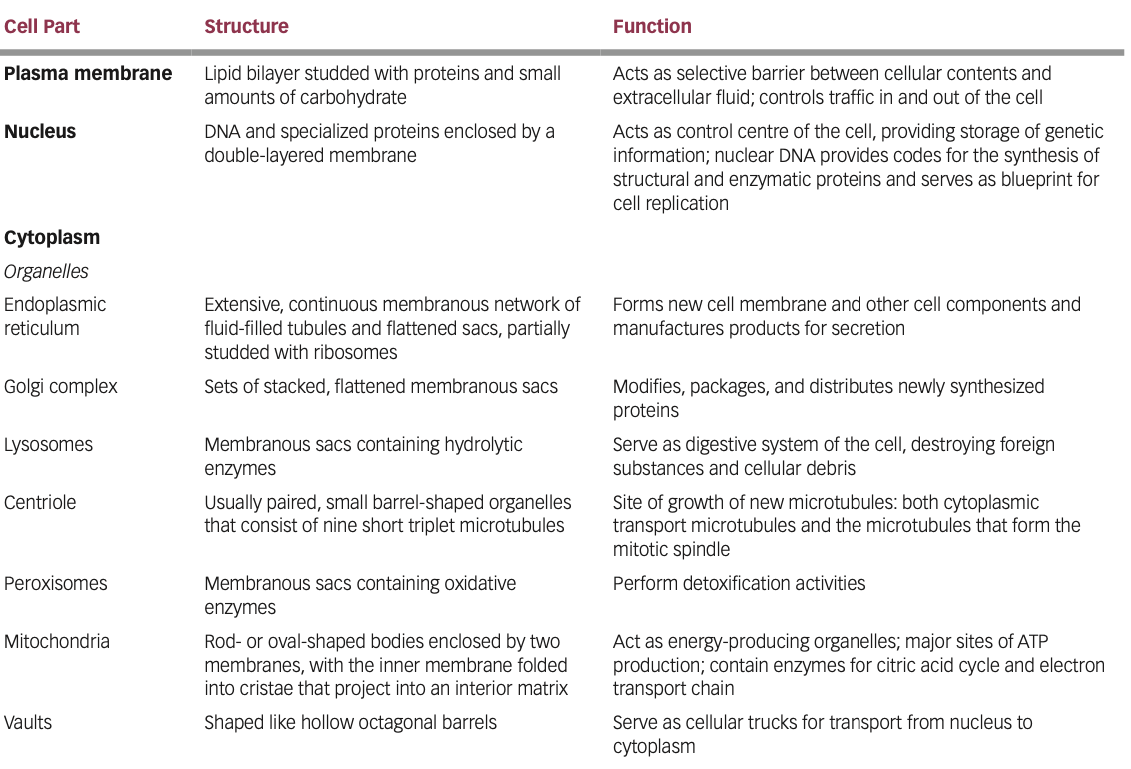
\includegraphics[scale=0.85]{cells1}
\end{figure}
\begin{figure}[htbp!]
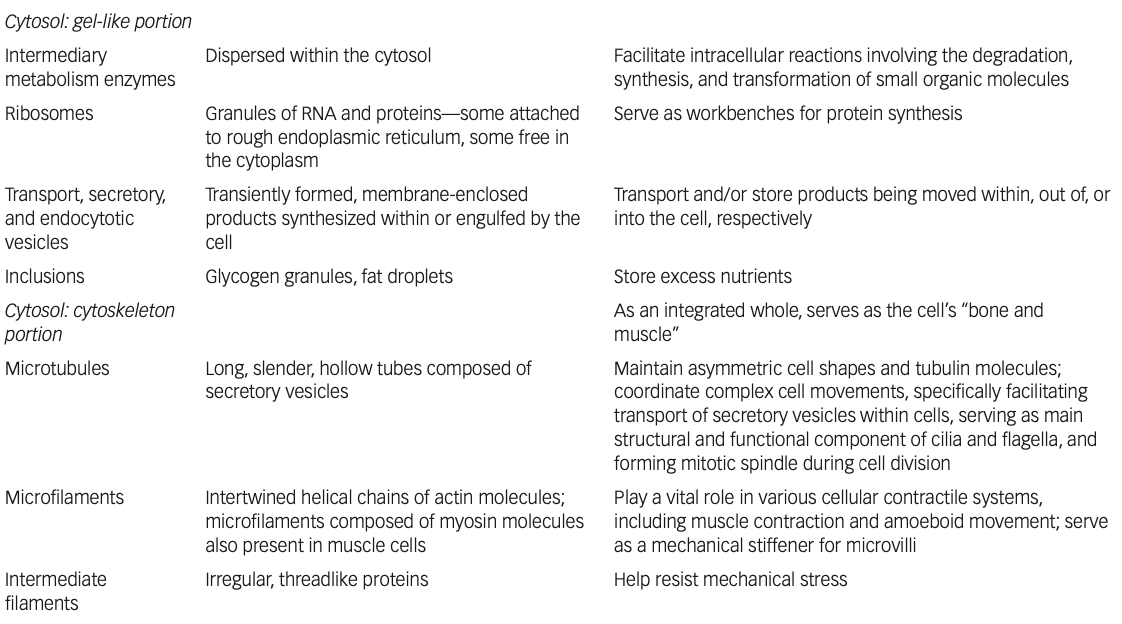
\includegraphics[scale=0.85]{cells2}
\end{figure}
\\
\subsection{Cellular Metabolism}
\begin{itemize}
\item \textbf{Intermediary metabolism }refers collectively to the large set of of chemical reactions inside the cell that involve degradation, synthesis, and transformation of of small organic molecules, such as sugars, amino acids, and fatty acids. 
\item \textbf{Anabolic} processes favour the synthesis of molecules 
\item \textbf{Catabolic} processes favour the breakdown of complex molecules to simple ones
\item Source of energy for body is stored in carbon bonds in food
\item The body converts the bonds into high energy \textbf{adenosine triphosphate (ATP) }bonds
\end{itemize}
\subsubsection{ATP Production}
There are 3 chemical pathways for ATP production:
\begin{itemize}
\item Substrate Level Phosphorylation
\item Anarobic Glycolosis
\item Aerobic Glycolosis
\end{itemize}
Follow 4 steps:
\begin{enumerate}
\item Glycolosis
\item Decarboxylation of Pyruvate
\item Tricarboxylic Acid Cycle
\item Electron Transport Chain (ETC)
\end{enumerate}
Ideally, 1 glucose would produce 38 ATP
\begin{itemize}
\item Assumes no energy is required in process
\item ETC runs at 100 \% efficiency
\end{itemize}
ATP is then used for the following:
\begin{itemize}
\item Synthesis of New Energy Compounds
\item Membrane Transport
\item Mechanical Work
\end{itemize}

\subsection{Plasma Membrane}
The survival of every cell depends on the maintenance of intracellular contents unique for that cell type. This difference in composition is maintained by by the plasma membrane, an extremely thin layer of lipids and proteins that forms the outer boundary of every cell and encloses the intracellular contents. The plasma membrane plays an active role in determining cell composition by selectively permitting specific cells to pass between the cell and its environment. It also maintains differences in ion concentrations between a cell's interior and exterior.

\subsubsection{Structure and Composition}
The plasma membrane consists of mostly lipids, proteins, and some carbohydrates. 
\begin{itemize}

\item \textbf{Phospholipids:} Have a polar, elecrically charged head, negatively charged phosphate group, and two fatty acid tails
\begin{itemize}
\item \textbf{Hydrophillic: }Water loving polar end; interacts with water molecules
\item \textbf{Hydrophobic: }Water fearing non-polar end; does not mix with water
\end{itemize}
\item \textbf{Lipid Bilayer:} Formed by phospholipids
\begin{itemize}
\item Cholesterol helps to stabilize the bilayer
\item Membrane proteins are attached / inserted into the bilayer
\item Fluid nature, but structural integrity; flexible to still be able to change shape
\item Known as the fluid mosaic model
\\ \\
\item Has three important functions:
\begin{enumerate}
\item Forms basic structure of the membrane; "picket around a fence"
\item Hydrophobic barrier serves as a barrier to passage of water-soluble substances between the ICF and ECF; helps maintain different mixtures and concentrations of solutes inside the cell
\item Responsible for fluidity of membrane
\end{enumerate}
\end{itemize}
\item \textbf{Membrane Proteins:} Various membrane proteins have different functions
\begin{itemize}
\item \textbf{Water Filled Pathways / Channels}
\begin{itemize}
\item Water soluble substances small enough can pass through without contact with hydrophobic interior
\item Selectively attract / repel ions
\item Adapt shape in response to control mechanisms
\end{itemize}
\item \textbf{Carrier Molecules}
\begin{itemize}
\item Transfer specific substances across that are unable to cross on their own
\end{itemize}
\item \textbf{Docking Marker Acceptors}
\begin{itemize}
\item Bind with secretory vesicles
\item When stimulatory signals trigger fusion with IC membrane it opens up
\end{itemize}
\item \textbf{Membrane Bound Enzymes}
\begin{itemize}
\item Control specific cell reactions
\end{itemize}
\item \textbf{Receptor Sites}
\begin{itemize}
\item Bind with things in cell environment that triggers events
\end{itemize}
\item \textbf{Cell Adhesion Molecules}
\begin{itemize}
\item Protrude from surface to form loops / hooks to grip to each other / connect tissues
\end{itemize}
\item \textbf{Other}
\begin{itemize}
\item Important for self recognition
\end{itemize}
\end{itemize}
\item \textbf{Self Recognition}
\begin{itemize}
\item Unique combinations of sugar chains projected from surface membrane serve as identity markers
\item Surface markers define boundaries to tissue growth; cancer ignores this
\end{itemize}
\end{itemize}


\subsection{Cell-to-Cell Adhesions}
Plasma membranes participate in cell-to-cell adhesions. Cells are held together by 3 different means:
\begin{itemize}
\item Extracellular Matrix
\item Cell Adhesion
\item Specialized Cell Junctions
\end{itemize}
\subsubsection{Biological Glue (Extracellular Matrix)}
\begin{itemize}
\item Holds together cells as a meschwork of fibrous proteins embedded in gel like water substances composed of complex carbohydrates
\item Gel provides a pathway for diffusion of nutrients, wastes, and other soluble traffic between blood and tissue
\item There are three main protein fibres
\begin{itemize}
\item \textbf{Collagen: }Cable like structures that provide tensile strength; scurvy weakens this
\item \textbf{Elastin: }Rubber like protein which can expand and contract; commonly found in lungs
\item \textbf{Fibronectin:} Promotes adhesion; holds cells in position
\end{itemize}
\item ECM is secreted by local cells, most by fibroplasts
\item Specialized composition; different, depending on cells 
\item Helps regulate behaviour and functions of cells (only circulating blood cells are designed to function without connecting to ECM)
\end{itemize}

\subsubsection{Cell Junctions}

\begin{itemize}

\item \textbf{Desmosomes}
\begin{itemize}
\item Act like spot rivets, anchoring adjacent non-touching cells 
\item Consists of two components 
\begin{itemize}
\item A pair of dense, button-like cytoplasmic thickenings known as plaque, located on the inner surface of each of the two adjacent cells
\item  Strong glycoprotein filaments con- taining cadherins (a type of CAM) that extend across the space between the two cells and attach to the plaque on both side
\end{itemize}
\item Most common in heart , uterus, skin that requires stretching
\end{itemize}

\item \textbf{Tight Junctions }
\begin{itemize}
\item Cells make direct contact and bind together sealing passageway between the two cells 
\item Found primarily at sites of epithelial tissue, like digestive tracts
\item Impermeability prevents material from passing between two cells; prevents undesirable leaks
\item "Kiss" sites where membrane is fused
\end{itemize}

\item \textbf{Gap Junctions}
\begin{itemize}
\item Gap in between cells by small tunnels formed by connexons
\item Connexons formed by 6 proteins arranged in hollow-like structure
\item Used as communicating junctions 
\item Allow small water soluble particles to pass, but not large ones
\item Abundant in cardiac and smooth muscle 
\item Helps transmit electrical signals and small signalling molecules 
\end{itemize}

\end{itemize}

\subsection{Overview Membrane Transport}
Anything that passes between a cell and the surrounding extracellular fluid must be able to penetrate the plasma membrane
Permeability refers to whether a substance can cross the membrane. The plasma membrane is \textbf{selectively permeable} as it permits some substances but restricts others. Two factors decide whether substances are permitted:
\begin{enumerate}
\item Relative Solubility of the Particle in Lipid
\item Size of the Particle
\end{enumerate}






\subsection{Unassisted Membrane Transport}
Molecules (or ions) that can penetrate the plasma membrane on their own are passively driven across the membrane by two forces: diffusion down a concentration gradient and/or movement along an electrical gradient.

\begin{itemize}
\item \textbf{Passive Diffusion of Particles}
\begin{itemize}
\item Molecules are always in constant motion; more likely to distribute
\item Spreading is called \textbf{diffusion}; difference in concentration is called \textbf{concentration gradient}
\item Steady state is dynamic equilibrium
\end{itemize}

\item \textbf{Passive Diffusion of Ions}
\begin{itemize}
\item Cations move towards negatively charged areas
\item Anions move toward positively charges areas
\item Electrical gradient promotes movement of ions 
\item Electrochemical gradient is combination of electrical / concentration gradient
\end{itemize}

\item \textbf{Osmosis}
\begin{itemize}
\item Water readily permeates membrane
\item Water moves from low concentration of solute to high concentration through semi-permeable membrane
\item Water moves down its own gradient
\item Three types of Osmosis
\begin{itemize}
\item \textbf{ Penetrating Solute:}
\begin{itemize}
\item Solute moves down concentration gradient, water balances volumes
\item Ceases when solute concentration balanced
\end{itemize}
\item \textbf{Non-Penetrating Solute:}
\begin{itemize}
\item Water moves to higher concentration until solute concentration balanced
\item Ending volumes change
\end{itemize}
\item \textbf{Pure Water with Non-Penetrating}
\begin{itemize}
\item Water moves until hydrostatic pressure balances osmotic pressure
\item Osmotic pressure is monitored to balance ECF and ICF
\end{itemize}
\end{itemize}
\item \textbf{Tonicity:} The effect a solution has on cell volume
\begin{itemize}
\item \textbf{Isotonic:} Same concentration of non-penetrating solutes as normal body cells
\item \textbf{Hypotonic:} Below-normal concentration of nonpenetrating solutes
\item \textbf{Hypertonic:} Above-normal concentration of nonpenetrating solute
\end{itemize}
\end{itemize}

\end{itemize}


\subsection{Assisted Membrane Transport}
For large, poorly lipid-soluble particles, they require deliberate transportation of essential nutrients (e.g. glucose, amino acids, etc.)
\begin{itemize}

\item \textbf{Carrier Mediated Transport:}
\begin{itemize}
\item Span the membrane, can flip flop to bring things in or back out 
\item Three important characteristics to determine material and amount to be transferred:
\begin{enumerate}
\item \textbf{Specificity}
\begin{itemize}
\item Carrier proteins are geared to transport specific substances
\end{itemize}
\item \textbf{Saturation}
\begin{itemize}
\item Limited number of carrier bonding sites
\item There is a transport maximum ($T_m$)
\item Rate of transport is directly related to concentration until $T_m$ is reached
\end{itemize}
\item \textbf{Competition}
\begin{itemize}
\item Different closely related compounds compete for same carrier
\end{itemize}
\end{enumerate}
\end{itemize}

\item \textbf{Active of Passive Transport:}
\begin{itemize}

\item \textbf{Facilitated Diffusion}
\begin{itemize}
\item Glucose into cell; not polar, thus not lipid soluble
\item High concentration causes net to go inwards, as passengers more likely to bind on the outside
\end{itemize}

\item \textbf{Active Transport}
\begin{itemize}
\item Involves protein carrier and usually ATP as energy source
\item ATP is required to modify affinity for bonding
\item \textbf{Phosphorylation} causes binding site to have greater affinity for passengers on low concentration side
\item Carrier flips, dephosphorylates, and passenger is released
\item Frequently called "pumps"
\item $Na^+$ - $K^+$ pump plays important roles
\begin{itemize}
\item Establishes $Na^+$ and $K^+$ concentration gradients across the plasma membrane of all cells
\item Helps regulate cell volume by controlling the concentra- tions of solutes inside the cell
\item Energy used to run the $Na^+$ - $K^+$  pump also indirectly serves as the energy source for the cotransport of glucose and amino acids across intestinal and kidney cells
\end{itemize}
\end{itemize}

\item \textbf{Secondary Active Transport}
\begin{itemize}
\item Glucose transported from lumens of intestines and kidneys are different than glucose facilitated diffusion
\item Instead it relies on cotransport luminal carriers
\item Carriers have one site for $Na^+$ and one for $K^+$
\item When $Na^+$ is binded, affinity for glucose is increased
\item Types of transport
\begin{itemize}
\item \textbf{Primary:} Energy is directly expended
\item \textbf{Secondary:} Doesn't use energy directly, second hand energy   of an ion concentration gradient
\end{itemize}
\end{itemize}
\end{itemize}


\item \textbf{Vesicular Transport}
\begin{itemize}
\item For larger molecules, requires energy expenditure to form vesicle and movement within
\item \textbf{Endocytosis:} Transport into the cell
\begin{itemize}
\item Once inside, endocytosis vesicles will either fuse with lysosomes to degrade and release contents into ICF or travel across the cell and release by exocytosis 
\item There are three types:
\begin{enumerate}
\item \textbf{Pinocytosis}
\begin{itemize}
\item Small droplet of ECF is internalized, a pouch is formed by membrane deforming coat proteins
\item Dynamin is a specialized protein to cut the endocycotic vesicle from the membrane
\end{itemize}
\item \textbf{Receptor Mediated Endocytosis}
\begin{itemize}
\item Highly selective process that allows cells to import needed cells 
\item Triggered by a protein / binding of a specific molecule 
\item Some viruses, such as HIV and flu virus take advantage of this
\end{itemize}
\item \textbf{Phagocytosis}
\begin{itemize}
\item Much less common, large multimolecular particles are internalized 
\item Lysosomes fuse with this internalized vesicle where they safely attack stuff
\end{itemize}
\end{enumerate}
\end{itemize}
\item \textbf{Exocytosis:} Transport out of the cell
\begin{itemize}
\item Opposite of exocytosis 
\item Vesicle fuses with the membrane, opens up and releases its content into exterior
\item Materialized packages for transport by the endoplasmic reticulum and golgi complex are externalized by exocytosis
\item Provides mechanism for secreting large polar molecules that are unable to cross membrane, contents are specific and released only on receipt of appropriate signals 
\item Allows cells to add channels, carriers, receptors to membrane
\end{itemize}



\end{itemize}

\item \textbf{Secretory Vesicles}
\begin{itemize}
\item Products of golgi apparatus collected at dilated edges of sacs, which pinches them off
\item Each surface protein marker serves as a specific docking marker
\item Secretory vesicles bud off golgi vesicles and fuse only with the membrane to prevent damage to the organelles
\item Contents never come into contact with cytosol
\end{itemize}

\end{itemize}

\subsection{Selective Permeability of the Membrane}

\subsubsection{Separation of Charges }
\begin{itemize}
\item \textbf{Membrane Potential:} Difference in electrical potential cause by difference in number of cations / anions between ECF and ICF 
\begin{itemize}
\item Can be harnessed to do work
\item When this changes, movement across current
\item $V = I/R$; $R$ determined by intrinsic properties of membrane
\end{itemize}
\end{itemize}

\subsubsection{Concentration / Permeability of Ions }
\begin{itemize}
\item Excitable tissues produce rapid transient changes in membrane potential serving as electrical signals
\item Resting membrane potential is when membrane is not transmitting signals 
\item Ions affecting membrane potentials ($Na^+$, $K^+$) and ions
\item $Na^+ $ more in the ECF, $K^+$ more in ICF
\item Knowing percentages of each type of ion allows us to analyse the effects of $K^+$ alone, $Na^+$ alone, and both together
\item Electrical gradient for cations are always toward the negative side

\end{itemize}
\begin{enumerate}
\item \textbf{Effect of Movement of $K^+$}
\begin{itemize}
\item ICF $>$ ECF, therefore concentration favours outside the cell
\item As $K^+$ leaves, ICF becomes negatively charged by cations that are unstable to leave, establishing membrane potential
\item Two forces opposing each other, creating \textbf{equilibrium potential}
\item More $K^+$ in ICF but it would stop moving out
\item $E_{K^+} = -90 mV$; negative means inside is -90 to the outside 
\item Equilibrium potential an be calculated with Nernst Equation
$$ E = 6I \log \frac{C_o}{C_i} = 6 \frac{RT}{zF} \log \frac{C_{ECF}}{C_{ICF}}$$
\end{itemize}
\item \textbf{Effect of $Na^+$ Alone}
\begin{itemize}
\item Buildup of $Na^+$ inside concentration gradient, negative $Cl^-$ outside
\item Electrical gradient balances concentration gradient 
\item $E_{Na^+} = 60 mV $
\end{itemize}
\item \textbf{Concurrent $Na^+$ and $K^+$}
\begin{itemize}
\item $K^+$ greater effect because greater permeability; general rule for all ions
\item $Na^+$ neutralizes part of its effects
\item $-20 mV$ is typical resting potential 
\end{itemize}
\end{enumerate}
\begin{itemize}
\item Chloride Movement at Resting
\begin{itemize}
\item High concentration in ECF, anion, resting potential at -70 mV
\item Membrane potential drives $Cl^-$ movement alone so no pumps exist, permeability allows it to diffuse at equilibrium
\item Electrochemical gradient outwards balances inward concentration gradient
\end{itemize}
\end{itemize}

\subsubsection{Depolarization and Hyperpolarization}
\begin{itemize}
\item \textbf{Polarization: }Neurons typically at -70 mV; either charges positively would be polarized
\item \textbf{Depolarization: }Movement in positive direction, or upward on recording device
\item \textbf{Repolarization:} Return to resting potential
\item \textbf{Hyperpolarization:} Membrane is more polarized than resting potential, moves even further from $0V$ becoming more negative
\end{itemize}

\subsubsection{Electrical Signals and Ion Movement}
\begin{itemize}
\item Net inward = positive, then depolarized, upward deflection
\item Net outward = negative, then hyperpolarized, downwards deflection
\item \textbf{Leak Channels:} Open all the time, unregulated leakage of chosen ions
\item \textbf{Gated Channels:} Can alternately be closed or opened; closing results from 3-D configuration
\begin{itemize}
\item Voltage
\item Chemical
\item Mechanical
\item Thermal
\end{itemize}
\end{itemize}
There are two types of potential
\begin{itemize}
\item \textbf{Graded Potential:} Short distance
\item \textbf{Action Potential:} Long distance
\end{itemize}

\subsection{Action Potentials}
Action potentials are brief, rapid, large changes in membrane potential where potential actually reverses (inside becomes more positive). It involves only a portion of the total excitable cell membrane. They also do not decrease in strength across the cell membrane
\subsubsection{Reversal of Membrane Potential}
\begin{itemize}
\item Graded potential changes can initiate an action potential before the graded change dies off
\item Graded potential by electrical / chemical means depolarizes areas where action potentials can take place 
\item Process
\begin{enumerate}
\item Triggering event causes the membrane to depolarize from resting -70 mV until it reaches threshold potential 
\item Threshold potential between -50 and -55 mV is where explosive depolarization takes place
\item Membrane re-polarizes dropping back to resting
\item Brief hyper-polarization at end of phase
\end{enumerate}
\item An action potential lasts 1 ms, between 0 to +30 mV is called overshoot
\item \textbf{Voltage Gated Membrane Channel}
\item $Na^+$
\begin{itemize}
\item Small distortions in channel shape induced by changes can cause them to flip to another conformation
\item Consists of activation gate (opens/closes like a door) and inactivation gate (ball and chain sequence of amino acids guarding channel)
\item Membrane potential determines conformation
\end{itemize}
\item $K^+$
\begin{itemize}
\item Also has 3 conformations 
\item Consists of 4 individual subunits
\item Rather than distinct activation and in activation gates 
\item Instead electrical fields change conformation of the subunits, which determines if $K^+$ can flow through
\end{itemize}
\item \textbf{Changes in Permeability and Ion Movement During an Action Potential}
\begin{itemize}
\item At -70 mV all voltage gated$Na^+$ and $K^+$ channels are closed but capable of opening 
\item When action potential begins depolarizing towards threshols, voltage gated $Na^+$ opens
\item $Na^+$ becomes 600 than more permeable to $Na^+$ than $K^+$, attempt to drive $Na^+$ equilibrium of +60 mV
\item When gate opens, conformation allows inactivation fate to slowly bind 
\item Remains inactivated until membrane potential is resting
\item As $Na^+$ inactivation begins, a spin of $K^+$ begins; $K^+$ opens delay after initial depolarization to threshold
\begin{enumerate}
\item Rapid opening of $Na^+$ activation gates,$Na^+$ enters for positive peak
\item Slow closing of inactivation gates to prevent further $Na^+$ from entering\item Slow opening of $K^+$ gates helping to restore peak to resting potential
\end{enumerate}
\item AS voltage returns to normal $Na^+$ and $K^+$ channels close 
\item Slow closing of  $K^+$ gates cause more $K^+$ to leave than necessary causing hyper-polarization 
\end{itemize}
\end{itemize}



\subsubsection{Restoration of Concentration}
\begin{itemize}
\item $Na^+$ - $K^+$ pump restore ions to original concentration
\item Only 1 of 100000 $K^+$ ions leave cell during action potential; $Na^+$ moves more
\item Still there is more $K^+$ in ICF than $Na^+$ in ECF
\item $Na^+$ - $K^+$ crucial to maintain gradients long term
\end{itemize}

\subsubsection{Propagation of Action Potential}
\begin{itemize}
\item Mechanisms exist to conduct / spread action potential 
\item Neurons consist of 
\begin{itemize}
\item Cell body
\item Dendrites - up to 400000
\item Axon
\end{itemize}
\end{itemize}

\subsubsection{Conduction via Nerve Fibre}
\begin{itemize}
\item When action potential at axon hillcock, impulse automatically conducted throughout nerve without further stimulation
\item There are two methods of conduction
\item \textbf{Contiguous conduction}
\begin{itemize}
\item Spread of action down membrane of the length of axon
\item Must spread to depolarized area which have reached threshold, accomplished by local current flow 
\item Flow of opposite charges attract opening $Na^+$ gates at inactive areas
\item Propagation is non-decremental
\end{itemize}
\end{itemize}

\subsubsection{One-Way Propagation}
\begin{itemize}
\item Oscillations are prevented by \textbf{refractory period} (makes it forward only)
\begin{itemize}
\item New events cannot occur in regions that have just undergone an action potential
\item Two part refractory period
\begin{enumerate}
\item \textbf{Absolute Refractory Period:} Period which membrane is completely unresponsive to further change; must reset to resting potential
\item \textbf{Relative Refractory Period:} Time where a triggering event considerably stronger is necessary to generate action potential
\end{enumerate}
\item By the time refractory period occurs, action potential has already propagated thus preventing backwards flow
\end{itemize}
\end{itemize}

\subsubsection{All-or-None Fashion }
\begin{itemize}
\item If any part is depolarized to threshold, action potential is relayed in an undiminished fashion
\item Stronger event does not generate a potential 
\item If event does not reach threshold, nothing happens
\end{itemize}

\subsubsection{Strength of Stimulus and Frequency of Action Potentials}
\begin{itemize}
\item To differentiate between stimuli, frequency of action potentials vary
\item Larger potential generates greater number of action potentials
\item Strength also affects number of neurons reading threshold, increasing total info sent 
\item Speed of action potential depends on if fibre is myelinated and its diameter
\end{itemize}

\subsubsection{Myelination and Speed of Conduction}
\begin{itemize}
\item Covered with myelins 
\begin{itemize}
\item 80 \% lipid, 20 \% protein
\item Act as an insulator preventing leakage because ions cannot permeate barrier
\item Not actively part of cell but wrap themselves around
\end{itemize}
\item Myelin types
\begin{itemize}
\item Brain, Spinal Cord
\end{itemize}
\item Nodes of Ranvier run between myelin sheets, only here can action potential spread
\begin{itemize}
\item Separated by space
\item Conducts around 50x faster
\item Conserves energy
\end{itemize}
\end{itemize}
\subsubsection{Fibre Diameter and Velocity of Action Potential}
\begin{itemize}
\item Increase diameter decreases resistance 
\item Types and Speeds
\begin{itemize}
\item Skeletal - large; travel at 127 m/s
\item Digestive - small; travel at 0.7 m/s
\end{itemize}
\item of myelinated increased efficiency and need for enormous fibres does not exist
\end{itemize}
\subsection{Graded Potentials}
Graded potentials are local changes in membrane potential that occur in varying grades or degrees of magnitude or strength.
\begin{itemize}
\item \textbf{Triggering Events}
\begin{itemize}
\item Caused by specific triggering events that cause gated ion channels to open in a specialized region of the cell membrane
\item Most commonly $Na^+$ gated channels open allowing $Na^+$ to travel down concentration gradient
\item Results in depolarization towards positive $Na^+$ equilibrium
\item Magnitude related to strength of event
\end{itemize}
\item \textbf{Graded Potentials and Passive Currents}
\begin{itemize}
\item When it occurs locally in an nerve, only excited membrane is called; active area more positive than rest area
\item Flow of ions is called current, positive on ECF goes toward $Na^+$ gate; moves away in ICf
\item Active areas spread in all directions to inactive areas
\item Amount of current that flows between two areas depend on difference in potential and on resistance; body lipids have high resistances; ICF and ECF have low resistances
\end{itemize}
\item \textbf{Graded Potentials and Current Loss}
\begin{itemize}
\item Current is lost through open channels on the membrane
\item The signal is decremental, decreases from initial site until it is not a graded potential
\item Limited signalling distance
\item Useful for 
\begin{itemize}
\item Post synaptic potentials
\item Receptor potentials
\item End plate potentials
\item Pacemaker potentials
\item Slow wave potentials
\end{itemize}
\item Excitable cells usually only produce one of these signals
\end{itemize}
\end{itemize}
\subsection{Synapses and Neuronal Integration}
\begin{itemize}
\item When action reaches axon terminals, they release a chemical messenger
\item Neurons terminate at three different locations 
\begin{enumerate}
\item \textbf{Muscle:} Neuron \textbf{innervates the muscles}
\item \textbf{Gland: }Tells it to secrete
\item\textbf{Another Neuron: }Convey electrical message
\end{enumerate}
\item Junction between two neurons is called a synapse
\end{itemize}
\subsubsection{Synapses}
\begin{itemize}
\item Usually between an axon terminal of one neuron and dendrite of another
\item Pre-synaptic neuron conducts action potential towards synapse ending with a synaptic knob 
\item Synaptic knob contains synaptic vesicles, which store chemical neuromessenger
\item Action between pre and post neuron is called synaptic cleft
\item Pre and post don't touch, excitation occurs by chemical means, moves in 1 direction 
\end{itemize}
\subsubsection{Neurotransmitters / Signal}
\begin{itemize}
\item What happens at the synapse?
\begin{enumerate}
\item Action potential is propagated to axon terminal, where it opens a $Ca^{2+}$ voltage gated channels 
\item $Ca^{2+}$ is highly concentrated in ECF, electrical gradient is also inward, ion flows into synaptic knob through channels
\item  $Ca^{2+}$ induces release of a neurotransmitter of some synaptic vesicles into synaptic cleft 
\item Neurotransmitter diffuses across cleft and binds with protein receptors in sub-synaptic membrane
\item Binding triggers opening of specific ion channels on post synaptic neuron, thus changing its permeability
\end{enumerate}
\item Since post synaptic depends on a chemical messenger from pre-synaptic neuron, it is one way
\end{itemize}
\subsection{Synapse Behaviour}
\begin{itemize}
\item Neurons aren't constrained to one type of neurotransmitter
\begin{itemize}
\item Neuroactive peptides and other neuroactive molecules can be contained in the same neuron
\item Mature neurons commonly contain one small molecule transmitter and one or more peptides
\end{itemize}
\item Neurotransmitter binding changes ion permeability
\item Two types of synapses
\begin{itemize}
\item \textbf{
Excitatory Synapses}
\begin{itemize}
\item Response to neurotransmitter binding to receptor is the opening of non-specific cotton channels 
\item Difference to earlier passages is the simultaneous increase of permeability for both $Na^+$ and $K^+$ 
\item At resting:
\begin{itemize}
\item $K^+$: Concentration gradient favours movement outwards from post synaptic neuron
\item $Na^+$: Concentration and electrochemical gradient favour movement into post-synaptic neuron
\end{itemize}
\item At excitatory state:
\begin{itemize}
\item $K^+$: Few move in
\item $Na^+$: Lots move in
\end{itemize}
\item Effect is that potential is closer to threshold and is more easily excitable
\item Called \textbf{excitatory post-synaptic potential}
\end{itemize}
\item \textbf{Inhibitory Synapses}
\begin{itemize}
\item Binding of different released neurotransmitter increases permeability of either $K^+$ or  $Cl^-$ resulting in small hyper-polarization in post synaptic neuron
\item Makes neuron less likely to reach threshold 
\item Said to be \textbf{inhibitory post-synaptic potential}
\end{itemize}
\end{itemize}
\item EPSP and IPSP arise from chemicals unlike action potentials which result from voltage gated channels 
\end{itemize}
\subsubsection{Receptor Combinations}
\begin{itemize}
\item Each synapse always releases the same neurotransmitter and its sub synaptic receptors always lead some change in permeability
\item Different synapses can have different receptor behaviours to the same neurotransmitter
\item Synapses can release more than one neurotransmitter at the same axon terminal 
\end{itemize}
\subsubsection{Neurotransmitter Removal}
\begin{itemize}
\item EPSP / IPSP lasts as long as neurotransmitter is binded
\item Once purpose is served, it can be removed by:
\begin{enumerate}
\item Diffusing away from the synaptic cleft
\item Be inactivated by specific enzymes within the sub-synaptic membrane
\item Be taken back into axon terminals by transport mechanism in the pre-synaptic membrane
\end{enumerate}
\end{itemize}
\subsubsection{Grand Post Synaptic Potential}
\begin{itemize}
\item EPSPs and IPSPs are graded potentials
\item Signal is received from many pre-synaptic neurons
\item Total potential is known as \textbf{grand post-synaptic potential} $GPSP = \sum IPSP + \sum EPSP$
\item Threshold can be reached with two methods
\begin{enumerate}
\item Temporal Summation
\begin{itemize}
\item Summing of several EPSPs occurring together because of successive firing of a single pre-synaptic neuron 
\item Amount of neurotransmitter released is directly related to frequency of pre-synaptic action potentials
\end{itemize}
\item \textbf{Spatial Summation }
\begin{itemize}
\item $EPSP_1 + EPSP_2$ reach threshold but neither alone
\item When different pre-synaptic  neurons concurrently activate several excitatory inputs
\end{itemize}
\end{enumerate}
\item \textbf{Cancellation: } When EPSPs and IPSPs hyperpolarize and depolarize and cancel out
\item \textbf{Importance of Post-Synaptic Neuronal Integration}
\begin{itemize}
\item EPSP depends on all pre-synaptic inputs to decide whether or not to pass on information
\item Dendrites are primarily processors of incoming information
\item System prevents small EPSP from releasing action potentials
\end{itemize}
\end{itemize}

\subsubsection{Action Potentials at Axon Hillcock}
\begin{itemize}
\item Axon Hillcock has the lowest threshold because it has the most $Na^+$ channels there
\item Much more responsive than dendrites or remainder of cell, which is why most action potential originates there
\end{itemize}


\subsection{Neuropeptides as Neuromodulators}
\begin{itemize}
\item Some neurons also release neuropeptides 
\item \textbf{Classic Neurotransmitters}
\begin{itemize}
\item Small rapid acting molecules that trigger opening of specific ion channels causing EPSPs or IPSPs within milliseconds
\end{itemize}
\item \textbf{Neuropeptides}
\begin{itemize}
\item Larger molecules made up anywhere from  2-40 amino acids
\item Synthesized in cell body endoplasmic reticulum and golgi complex and moved to axon terminals
\item Packaged in dense-core vesicles, not synaptic vesicles
\item Undergo exocytosis by $Ca^{2+}$ same as neurotransmitters
\item Some may function as neurotransmitters, others as neuromodulators
\end{itemize}
\item \textbf{Neuromodulators}
\begin{itemize}
\item Do not form EPSPs or IPSPs
\item Make long term changes subtly modulate action of synapse
\item Many have roles as hormones
\end{itemize}
\end{itemize}

\subsubsection{Pre-synaptic Inhibition or Facilitation}
\begin{itemize}
\item Another means other than neuromodulators that depresses / enhances synaptic effectiveness
\item If synaptic axon terminal is innervated by another axon terminal:
\begin{itemize}
\item If neurotransmitter is increased $\rightarrow$ pre-synaptic facilitation
\item If neurotransmitter is reduced $\rightarrow$ pre-synaptic inhibition
\end{itemize}
\item Modulatory neuron controls this by reducing $Ca^{2+}$ entry to the terminal
\end{itemize}

\subsubsection{Drugs, Diseases, and Transmission}
\begin{itemize}
\item \textbf{Drugs}
\begin{itemize}
\item Alter biological function of the organism
\item Those that affect nervous system alter synaptic mechanisms
\begin{itemize}
\item Altering synthesis / axonal transport / storage / release of a transmitter
\item Modifying neurotransmitter interaction with post-synaptic receptor
\item Influencing neurotransmitter reuptake / destruction
\item Replacing deficient neurotransmitter with substitute
\end{itemize}
\end{itemize}
\item \textbf{Parkinson's Disease}
\begin{itemize}
\item Deficiency of dopamine in basal nuclei
\end{itemize}
\item \textbf{Synaptic Transmission}
\begin{itemize}
\item\textbf{Stryclinc Toxin:} Clogs receptor sites
\item \textbf{Tetanus Toxin:} Prevents neurotransmitter release
\end{itemize}
\end{itemize}
\subsubsection{Neurons}
\begin{itemize}
\item \textbf{Convergence: }A post synaptic neuron is influenced by many cells
\item \textbf{Divergence: }A pre synaptic input influences many other neurons
\item Estimated 10 million neurons in the brain alone
\end{itemize}
\pagebreak


\section{Central Nervous System}

\subsection{Organization of the Nervous System}
The nervous system is organized into the central nervous system (CNS), peripheral nervous system (PNS)
\begin{itemize}
\item \textbf{Central Nervous System (CNS)}
\begin{itemize}
\item Brain and Spinal Cord
\end{itemize}
\item \textbf{Peripheral Nervous System (PNS)}
\begin{itemize}
\item Nerve fibres that carry information
\item \textbf{Afferent Division:} Carries info to CNS
\item\textbf{ Efferent Division: }Carries info to effector organs
\begin{itemize}
\item \textbf{Somatic Nervous System: } Nerve fibres of the motor neurons that supply the skeletal muscle
\item \textbf{Autonomic Nervous System (ANS): }Nerve fibres that innervate smooth muscle, cardiac muscle, and glands
\begin{itemize}
\item Sympathetic Nervous System
\item Parasympathetic Nervous System
\end{itemize}
\end{itemize}
\end{itemize}
\end{itemize}
There are three classes of neurons that make up the nervous system:
\begin{itemize}
\item \textbf{Afferent Neurons}
\begin{itemize}
\item At peripheral ending, a sensory receptor generates an action potential
\item No dendrites or pre-synaptic inputs
\item Propagate signals to spinal cord; typically found in PNS
\end{itemize}
\item\textbf{ Efferent Neurons}
\begin{itemize}
\item Primarily in PNS, cell body in CNS
\item Convey signals to efferent organs
\end{itemize}
\item \textbf{Interneurons}
\begin{itemize}
\item Entirely in CNS, 99 \% of neurons
\item Estimated 100 billion interneurons
\end{itemize}
\end{itemize}

\subsection{Central Nervous System}
The central nervous system has many important roles and functions:
\begin{itemize}
\item  Subconsciously regulate your internal environment by neural movements
\item Experience emotions
\item Voluntary control movement
\item Perceive / be conscious of yourself and surroundings
\item Thought and memory
\end{itemize}
The system is grouped as follows 
\begin{itemize}
\item Brain stem
\item Cerebellum
\item Forebrain
\begin{itemize}
\item Diencephalon
\begin{itemize}
\item Hypothalamus
\item Thalamus
\end{itemize}
\item Cerebrum
\begin{itemize}
\item Basal Ganglia
\item Cerebral Cortex
\end{itemize}
\end{itemize}
\end{itemize}


\subsection{Protection of CNS}
\begin{itemize}
\item\textbf{Glial Cells}
\begin{itemize}
\item 90 \% of cells in CNS, only half the volume of the brain
\item Do not initiate or conduct nerve impulses; communicate with neurons and between themselves via chemicals
\item Glue as they are CNS connective tissue and support neurons physically and metabolically
\item Four major types:
\begin{itemize}
\item \textbf{Astrocytes}
\begin{itemize}
\item Main connective tissue of cells; hold neurons together
\item Scaffolding around neurons during fetal brain development
\item Responsible for establishing brain-blood barrier
\item Brain injuries and neural scar formation
\item Neurotransmitter activity
\item Maintain proper ECF ion concentration in brain
\item Enhance synapse formation and strengthen synapse impulse transmission
\end{itemize}
\item \textbf{Oligodendrocytes}
\begin{itemize}
\item Form insulating myelin sheaths around axons
\end{itemize}
\item \textbf{Microglia}
\begin{itemize}
\item Immune cells in the CNS; wispy with loing branches that extend outwards
\item Can cause neurodegenerative diseases if too overzealous
\end{itemize}
\item \textbf{Epindymal}
\begin{itemize}
\item Like internal CNS cavities (brain and spinal cord) 
\item Contribute to cerebrospinal fluid formation
\end{itemize}
\end{itemize}
\end{itemize} 
\item \textbf{Protection of CNS}
\begin{itemize}
\item Skull and vertabral column
\item Meninges
\begin{itemize}
\item Protective / nourishing membranes between bone and tissue
\item 3 membranes
\begin{itemize}
\item Dura Mater
\item Arachnoid Mater
\item Pia Mater
\end{itemize}
\end{itemize}
\item Cerebrospinal fluid
\begin{itemize}
\item Acts as a cushion for the brain
\end{itemize}
\item Blood-brain barrier
\begin{itemize}
\item Highly sensitive membrane of endothelial cells; material exchange only through capillary walls
\end{itemize}
\end{itemize}
\end{itemize}



\subsection{Spinal Cord}
\begin{itemize}
\item Long slender cylinder of nerve tissue protected by the vertebral column
\begin{itemize}
\item \textbf{Vertebral Canal}
\begin{itemize}
\item \textbf{Paired Spinal Nerves: }Emerge from spinal cord between the protrusions of adjacent successive vertebrae
\item \textbf{Cauda Equina:} The paired nerve roots that descend far below end of the spinal cord
\end{itemize}
\item \textbf{Spinal Cord White Matter}
\begin{itemize}
\item Surrounds butterfly shaped gray matter
\end{itemize}
\item \textbf{Spinal Cord Gray Matter}
\begin{itemize}
\item \textbf{Dorsal Horn:} Carrying cell bodies of inter neurons and terminals of afferent neurons
\item \textbf{Lateral Horn: }Cell bodies of automatic efferent nerve fibres
\item \textbf{Ventral Horn: }Cell bodies of somatic efferent neurons
\end{itemize}
\item\textbf{ Spinal Nerves}
\begin{itemize}
\item Connect with each side of a spinal cord via dorsal and ventral root
\end{itemize}
\item \textbf{Peripheral Nervous System}
\begin{itemize}
\item Made of 31 spinal nerves and 12 cranial nerves
\end{itemize}
\end{itemize}
\item \textbf{Reflexes}
\begin{itemize}
\item Basic reflexes 
\item Acquired reflexes
\item Stretch reflexes
\item Withdrawal reflexes 
\end{itemize}
\end{itemize}



\subsection{Brain Stem}
All fibres must pass through stem if headed toward higher brain centres. Its functions include
\begin{enumerate}
\item Origin of most of cranial nerves
\item Control heart/blood circulation, respiration, and digestion
\item Regulates muscle reflexes for balance and posture
\item Reticular formation
\item Governs sleep

\end{enumerate}
\subsection{Thalamus and Hypothalamus}
Two divisions of the diencephalon
\begin{itemize}
\item \textbf{Thalamus}
\begin{itemize}
\item Relay station and synaptic integrating centre for preliminary sensory processing before these inputs go to the cortex
\end{itemize}
\item \textbf{Hypothalamus}
\begin{itemize}
\item Collection of specific nuclei and fibres underneath the thalamus 
\item Integrating centre for homeostatis functions and is an important link between autonomic nervous system and the endocrine system
\end{itemize}
\end{itemize}

\subsection{Cerebral Cortex}
Largest portion of brain, which is divided into two halves - left and right brain
\begin{itemize}
\item \textbf{Gray and White Matter in Cortex}
\begin{itemize}
\item Thin outer layer of gray matter
\item Thick center core of white matter
\item Gray matter integrates input info and starts output info and the white matter transmits these signals throughout the cortex because each area of the cortex may process different info that needs to be integrated together
\end{itemize}
\item \textbf{Layers and Columns}
\begin{itemize}
\item Organized into 6 layers based on cell types within
\item Layers organized into columns; neurons in each column function as a team
\end{itemize}
\item \textbf{Lobes}
\begin{itemize}
\item \textbf{Occipital: }Initial visual processing
\item \textbf{Temporal:} Initial sound processing
\item \textbf{Parietal:} Receiving and processing sensory input
\item \textbf{Frontal:} 3 main functions
\begin{itemize}
\item Voluntary motion
\item Speaking
\item Elaboration of thought
\end{itemize}
\end{itemize}
\item \textbf{Neuroplasticity and Regeneration of Brain Tissue}
\begin{itemize}
\item Brain has a degree of plasticity 
\item Higher plasticity in developmental years
\item When area of brain is damaged, neuron connections can change
\item Generation of new brain cells has also been proposed
\end{itemize}
\end{itemize}

\end{document}
